
%% bare_conf_compsoc.tex
%% V1.4b
%% 2015/08/26
%% by Michael Shell
%% See:
%% http://www.michaelshell.org/
%% for current contact information.
%%
%% This is a skeleton file demonstrating the use of IEEEtran.cls
%% (requires IEEEtran.cls version 1.8b or later) with an IEEE Computer
%% Society conference paper.
%%
%% Support sites:
%% http://www.michaelshell.org/tex/ieeetran/
%% http://www.ctan.org/pkg/ieeetran
%% and
%% http://www.ieee.org/

%%*************************************************************************
%% Legal Notice:
%% This code is offered as-is without any warranty either expressed or
%% implied; without even the implied warranty of MERCHANTABILITY or
%% FITNESS FOR A PARTICULAR PURPOSE! 
%% User assumes all risk.
%% In no event shall the IEEE or any contributor to this code be liable for
%% any damages or losses, including, but not limited to, incidental,
%% consequential, or any other damages, resulting from the use or misuse
%% of any information contained here.
%%
%% All comments are the opinions of their respective authors and are not
%% necessarily endorsed by the IEEE.
%%
%% This work is distributed under the LaTeX Project Public License (LPPL)
%% ( http://www.latex-project.org/ ) version 1.3, and may be freely used,
%% distributed and modified. A copy of the LPPL, version 1.3, is included
%% in the base LaTeX documentation of all distributions of LaTeX released
%% 2003/12/01 or later.
%% Retain all contribution notices and credits.
%% ** Modified files should be clearly indicated as such, including  **
%% ** renaming them and changing author support contact information. **
%%*************************************************************************


% *** Authors should verify (and, if needed, correct) their LaTeX system  ***
% *** with the testflow diagnostic prior to trusting their LaTeX platform ***
% *** with production work. The IEEE's font choices and paper sizes can   ***
% *** trigger bugs that do not appear when using other class files.       ***                          ***
% The testflow support page is at:
% http://www.michaelshell.org/tex/testflow/



\documentclass[conference,compsoc]{IEEEtran}
% Some/most Computer Society conferences require the compsoc mode option,
% but others may want the standard conference format.
%
% If IEEEtran.cls has not been installed into the LaTeX system files,
% manually specify the path to it like:
% \documentclass[conference,compsoc]{../sty/IEEEtran}





% Some very useful LaTeX packages include:
% (uncomment the ones you want to load)


\usepackage{listings}
\usepackage{xcolor}
\lstset{
  showstringspaces=false,
  commentstyle=\color{red},
  keywordstyle=\color{blue}
}

% *** MISC UTILITY PACKAGES ***
%
%\usepackage{ifpdf}
% Heiko Oberdiek's ifpdf.sty is very useful if you need conditional
% compilation based on whether the output is pdf or dvi.
% usage:
% \ifpdf
%   % pdf code
% \else
%   % dvi code
% \fi
% The latest version of ifpdf.sty can be obtained from:
% http://www.ctan.org/pkg/ifpdf
% Also, note that IEEEtran.cls V1.7 and later provides a builtin
% \ifCLASSINFOpdf conditional that works the same way.
% When switching from latex to pdflatex and vice-versa, the compiler may
% have to be run twice to clear warning/error messages.






% *** CITATION PACKAGES ***
%
\ifCLASSOPTIONcompsoc
  % IEEE Computer Society needs nocompress option
  % requires cite.sty v4.0 or later (November 2003)
  \usepackage[nocompress]{cite}
\else
  % normal IEEE
  \usepackage{cite}
\fi
% cite.sty was written by Donald Arseneau
% V1.6 and later of IEEEtran pre-defines the format of the cite.sty package
% \cite{} output to follow that of the IEEE. Loading the cite package will
% result in citation numbers being automatically sorted and properly
% "compressed/ranged". e.g., [1], [9], [2], [7], [5], [6] without using
% cite.sty will become [1], [2], [5]--[7], [9] using cite.sty. cite.sty's
% \cite will automatically add leading space, if needed. Use cite.sty's
% noadjust option (cite.sty V3.8 and later) if you want to turn this off
% such as if a citation ever needs to be enclosed in parenthesis.
% cite.sty is already installed on most LaTeX systems. Be sure and use
% version 5.0 (2009-03-20) and later if using hyperref.sty.
% The latest version can be obtained at:
% http://www.ctan.org/pkg/cite
% The documentation is contained in the cite.sty file itself.
%
% Note that some packages require special options to format as the Computer
% Society requires. In particular, Computer Society  papers do not use
% compressed citation ranges as is done in typical IEEE papers
% (e.g., [1]-[4]). Instead, they list every citation separately in order
% (e.g., [1], [2], [3], [4]). To get the latter we need to load the cite
% package with the nocompress option which is supported by cite.sty v4.0
% and later.





% *** GRAPHICS RELATED PACKAGES ***
%
\ifCLASSINFOpdf
   \usepackage[pdftex]{graphicx}
%   declare the path(s) where your graphic files are
%   \graphicspath{{../img/}{../jpeg/}}
%   and their extensions so you won't have to specify these with
%   every instance of \includegraphics
%   \DeclareGraphicsExtensions{.pdf,.jpeg,.png}
\else
  % or other class option (dvipsone, dvipdf, if not using dvips). graphicx
  % will default to the driver specified in the system graphics.cfg if no
  % driver is specified.
  % \usepackage[dvips]{graphicx}
  % declare the path(s) where your graphic files are
  % \graphicspath{{../eps/}}
  % and their extensions so you won't have to specify these with
  % every instance of \includegraphics
  % \DeclareGraphicsExtensions{.eps}
\fi
% graphicx was written by David Carlisle and Sebastian Rahtz. It is
% required if you want graphics, photos, etc. graphicx.sty is already
% installed on most LaTeX systems. The latest version and documentation
% can be obtained at: 
% http://www.ctan.org/pkg/graphicx
% Another good source of documentation is "Using Imported Graphics in
% LaTeX2e" by Keith Reckdahl which can be found at:
% http://www.ctan.org/pkg/epslatex
%
% latex, and pdflatex in dvi mode, support graphics in encapsulated
% postscript (.eps) format. pdflatex in pdf mode supports graphics
% in .pdf, .jpeg, .png and .mps (metapost) formats. Users should ensure
% that all non-photo figures use a vector format (.eps, .pdf, .mps) and
% not a bitmapped formats (.jpeg, .png). The IEEE frowns on bitmapped formats
% which can result in "jaggedy"/blurry rendering of lines and letters as
% well as large increases in file sizes.
%
% You can find documentation about the pdfTeX application at:
% http://www.tug.org/applications/pdftex





% *** MATH PACKAGES ***
%
%\usepackage{amsmath}
% A popular package from the American Mathematical Society that provides
% many useful and powerful commands for dealing with mathematics.
%
% Note that the amsmath package sets \interdisplaylinepenalty to 10000
% thus preventing page breaks from occurring within multiline equations. Use:
%\interdisplaylinepenalty=2500
% after loading amsmath to restore such page breaks as IEEEtran.cls normally
% does. amsmath.sty is already installed on most LaTeX systems. The latest
% version and documentation can be obtained at:
% http://www.ctan.org/pkg/amsmath





% *** SPECIALIZED LIST PACKAGES ***
%
%\usepackage{algorithmic}
% algorithmic.sty was written by Peter Williams and Rogerio Brito.
% This package provides an algorithmic environment fo describing algorithms.
% You can use the algorithmic environment in-text or within a figure
% environment to provide for a floating algorithm. Do NOT use the algorithm
% floating environment provided by algorithm.sty (by the same authors) or
% algorithm2e.sty (by Christophe Fiorio) as the IEEE does not use dedicated
% algorithm float types and packages that provide these will not provide
% correct IEEE style captions. The latest version and documentation of
% algorithmic.sty can be obtained at:
% http://www.ctan.org/pkg/algorithms
% Also of interest may be the (relatively newer and more customizable)
% algorithmicx.sty package by Szasz Janos:
% http://www.ctan.org/pkg/algorithmicx




% *** ALIGNMENT PACKAGES ***
%
%\usepackage{array}
% Frank Mittelbach's and David Carlisle's array.sty patches and improves
% the standard LaTeX2e array and tabular environments to provide better
% appearance and additional user controls. As the default LaTeX2e table
% generation code is lacking to the point of almost being broken with
% respect to the quality of the end results, all users are strongly
% advised to use an enhanced (at the very least that provided by array.sty)
% set of table tools. array.sty is already installed on most systems. The
% latest version and documentation can be obtained at:
% http://www.ctan.org/pkg/array


% IEEEtran contains the IEEEeqnarray family of commands that can be used to
% generate multiline equations as well as matrices, tables, etc., of high
% quality.




% *** SUBFIGURE PACKAGES ***
%\ifCLASSOPTIONcompsoc
%  \usepackage[caption=false,font=footnotesize,labelfont=sf,textfont=sf]{subfig}
%\else
%  \usepackage[caption=false,font=footnotesize]{subfig}
%\fi
% subfig.sty, written by Steven Douglas Cochran, is the modern replacement
% for subfigure.sty, the latter of which is no longer maintained and is
% incompatible with some LaTeX packages including fixltx2e. However,
% subfig.sty requires and automatically loads Axel Sommerfeldt's caption.sty
% which will override IEEEtran.cls' handling of captions and this will result
% in non-IEEE style figure/table captions. To prevent this problem, be sure
% and invoke subfig.sty's "caption=false" package option (available since
% subfig.sty version 1.3, 2005/06/28) as this is will preserve IEEEtran.cls
% handling of captions.
% Note that the Computer Society format requires a sans serif font rather
% than the serif font used in traditional IEEE formatting and thus the need
% to invoke different subfig.sty package options depending on whether
% compsoc mode has been enabled.
%
% The latest version and documentation of subfig.sty can be obtained at:
% http://www.ctan.org/pkg/subfig




% *** FLOAT PACKAGES ***
%
%\usepackage{fixltx2e}
% fixltx2e, the successor to the earlier fix2col.sty, was written by
% Frank Mittelbach and David Carlisle. This package corrects a few problems
% in the LaTeX2e kernel, the most notable of which is that in current
% LaTeX2e releases, the ordering of single and double column floats is not
% guaranteed to be preserved. Thus, an unpatched LaTeX2e can allow a
% single column figure to be placed prior to an earlier double column
% figure.
% Be aware that LaTeX2e kernels dated 2015 and later have fixltx2e.sty's
% corrections already built into the system in which case a warning will
% be issued if an attempt is made to load fixltx2e.sty as it is no longer
% needed.
% The latest version and documentation can be found at:
% http://www.ctan.org/pkg/fixltx2e


%\usepackage{stfloats}
% stfloats.sty was written by Sigitas Tolusis. This package gives LaTeX2e
% the ability to do double column floats at the bottom of the page as well
% as the top. (e.g., "\begin{figure*}[!b]" is not normally possible in
% LaTeX2e). It also provides a command:
%\fnbelowfloat
% to enable the placement of footnotes below bottom floats (the standard
% LaTeX2e kernel puts them above bottom floats). This is an invasive package
% which rewrites many portions of the LaTeX2e float routines. It may not work
% with other packages that modify the LaTeX2e float routines. The latest
% version and documentation can be obtained at:
% http://www.ctan.org/pkg/stfloats
% Do not use the stfloats baselinefloat ability as the IEEE does not allow
% \baselineskip to stretch. Authors submitting work to the IEEE should note
% that the IEEE rarely uses double column equations and that authors should try
% to avoid such use. Do not be tempted to use the cuted.sty or midfloat.sty
% packages (also by Sigitas Tolusis) as the IEEE does not format its papers in
% such ways.
% Do not attempt to use stfloats with fixltx2e as they are incompatible.
% Instead, use Morten Hogholm'a dblfloatfix which combines the features
% of both fixltx2e and stfloats:
%
% \usepackage{dblfloatfix}
% The latest version can be found at:
% http://www.ctan.org/pkg/dblfloatfix




% *** PDF, URL AND HYPERLINK PACKAGES ***
%
%\usepackage{url}
% url.sty was written by Donald Arseneau. It provides better support for
% handling and breaking URLs. url.sty is already installed on most LaTeX
% systems. The latest version and documentation can be obtained at:
% http://www.ctan.org/pkg/url
% Basically, \url{my_url_here}.




% *** Do not adjust lengths that control margins, column widths, etc. ***
% *** Do not use packages that alter fonts (such as pslatex).         ***
% There should be no need to do such things with IEEEtran.cls V1.6 and later.
% (Unless specifically asked to do so by the journal or conference you plan
% to submit to, of course. )


% correct bad hyphenation here
\hyphenation{op-tical net-works semi-conduc-tor}


\begin{document}
%
% paper title
% Titles are generally capitalized except for words such as a, an, and, as,
% at, but, by, for, in, nor, of, on, or, the, to and up, which are usually
% not capitalized unless they are the first or last word of the title.
% Linebreaks \\ can be used within to get better formatting as desired.
% Do not put math or special symbols in the title.
\title{MAC-based activity tracking using passive sniffing}


% author names and affiliations
% use a multiple column layout for up to three different
% affiliations
\author{\IEEEauthorblockN{Jetse Brouwer}
\IEEEauthorblockA{Delft university of technology\\Embedded Systems\\
Mekelweg 4, 2628 CD Delft\\
Email: j.brouwer-3@student.tudelft.nl}
\and
\IEEEauthorblockN{Niels Hokke}
\IEEEauthorblockA{Delft university of technology\\Embedded Systems\\
Mekelweg 4, 2628 CD Delft\\
Email: n.h.hokke@student.tudelft.nl}
}

% conference papers do not typically use \thanks and this command
% is locked out in conference mode. If really needed, such as for
% the acknowledgment of grants, issue a \IEEEoverridecommandlockouts
% after \documentclass

% for over three affiliations, or if they all won't fit within the width
% of the page (and note that there is less available width in this regard for
% compsoc conferences compared to traditional conferences), use this
% alternative format:
% 
%\author{\IEEEauthorblockN{Michael Shell\IEEEauthorrefmark{1},
%Homer Simpson\IEEEauthorrefmark{2},
%James Kirk\IEEEauthorrefmark{3}, 
%Montgomery Scott\IEEEauthorrefmark{3} and
%Eldon Tyrell\IEEEauthorrefmark{4}}
%\IEEEauthorblockA{\IEEEauthorrefmark{1}School of Electrical and Computer Engineering\\
%Georgia Institute of Technology,
%Atlanta, Georgia 30332--0250\\ Email: see http://www.michaelshell.org/contact.html}
%\IEEEauthorblockA{\IEEEauthorrefmark{2}Twentieth Century Fox, Springfield, USA\\
%Email: homer@thesimpsons.com}
%\IEEEauthorblockA{\IEEEauthorrefmark{3}Starfleet Academy, San Francisco, California 96678-2391\\
%Telephone: (800) 555--1212, Fax: (888) 555--1212}
%\IEEEauthorblockA{\IEEEauthorrefmark{4}Tyrell Inc., 123 Replicant Street, Los Angeles, California 90210--4321}}




% use for special paper notices
%\IEEEspecialpapernotice{(Invited Paper)}




% make the title area
\maketitle

% As a general rule, do not put math, special symbols or citations
% in the abstract
\begin{abstract}
Over the course of 5 days more than 1.2 million probe requests from over 91 thousand unique mac address were observed using low cost of the shelf hardware. Using this data, opening times and customer activity in a grocery store could be tracked. Using MAC address filtering the behaviour of individual customers and neighbouring residents is traceable.

\end{abstract}

% no keywords

% For peer review papers, you can put extra information on the cover
% page as needed:
% \ifCLASSOPTIONpeerreview
% \begin{center} \bfseries EDICS Category: 3-BBND \end{center}
% \fi
%
% For peerreview papers, this IEEEtran command inserts a page break and
% creates the second title. It will be ignored for other modes.
\IEEEpeerreviewmaketitle

\section{Introduction} 
Smart phones market penetration is ever increasing, with 68.8\% the Netherlands is the number eight based on smart phone ownership \cite{SmartPenetration}. While this increased connectivity can be of great convenience to the user, it might also supply other parties with a vast amounts of data. The goal of this paper is to explore the possibilities of tracking crowd activity as well as identifying and studying individuals by sniffing Wi-Fi packets transmitted by the smart phones. By placing a Wi-Fi sniffer at a crowded public place this papers aims to 1) monitor crowd activity over time 2) explore the feasibility of identifying and track behavior of individuals and 3) gather information about MAC randomization as a privacy enhancing feature.

\section{Method}

\subsection{Probe Requests}
To discover nearby access point (APs) the client has two options: It can either wait for an access point to announce it self by listening for beacons, or it can actively scan for nearby APs with the use of probe requests. Probe requests are a sub-type of 802.11 Management frames with the goal to discover near by access points. These probes can be either directed at a specific AP or broadcasted to any AP in the vicinity. On reception of such a request the AP sends a probe response with the parameters of the wireless network station such as supported data rates and channel usage. As the client only responds to beacons of networks it knows and wants to associate with, and we are also interested in customers who are not associated with nearby networks we will focus on capturing probe requests. According to the IEEE specification the header must always contain the following fields:
\begin{itemize}
\item frame control: frame type identifier
\item Address 1: Destination MAC address
\item Address 2: Source MAC address
\item Address 3: BSSID (only for directed probes)
\item Sequence control: Number to identify the probe
\end{itemize}


\subsection{Hardware setup}
As the authors had access to a postbox next to the entrance of a grocery store this location was chosen as the monitoring place. Due to the lack of a power outlet near the postbox an alternative power source such as a battery was needed. The chosen hardware-platform was the Raspberry Pi 3 due to its relatively low power consumption, affordability yet providing sufficient computational power.

During 'normal' use of a wireless network interface, the interface operates in 'managed mode' meaning only packets directly addressed to that specific network interface will be handled. To enable capturing of all packages within the network interfaces' reach it has to be put in 'monitor mode', which in our case required patched firmware as the Raspberry Pi 3 interface native did not support monitoring mode.

The Raspberry Pi 3 was equipped with Kali Linux, Debian-based Linux distribution designed for digital forensics and penetration testing. This as it includes patched firmware to enable monitor mode on the Raspberry Pi 3 among other commonly used software for sniffing data.

\subsection{Software setup}
The Raspberry Pi lacks a battery for the real-time clock, because of this the actual time will be lost at reboot. To synchronize the time an NTP client is started at the startup of the sniffer.

For capturing the packets Tshark (the command line interface implementation of Wireshark) was used. As we are only interested in probe requests we use a capture filter to reduce the amount of data to be stored. This filtering is done with the use of Tshark own capture filter syntax 'subtype probereq'. Tshark is setup to create a new pcap file every 5 minutes to lose at most 5 minutes of data corruption due to unexpected power loss. Besides exporting the PCAP files, Tshark is configured to also append the arrival time, MAC address and signal strength to a CSV for ease of use. 

As the interface can only monitor one channel at a certain time a script is utilized to change the Wi-Fi channel every 0.25 ms. This script was downloaded from \cite{chanhop.sh}


The script run at start up can be seen in \ref{listing:startup}.

\begin{figure}[h!]
    \centering
\begin{lstlisting}[language=bash,caption={mac\_tracker.sh}]

#!/bin/bash
echo 'Synchronizing date and  time'
ntpdate ntp0.nl.net

echo 'create dir and mount usb-stick'  
umount /dev/sda1
mkdir output
mount /dev/sda1 output/

echo 'setting wlan0 to monitoring mode'
airmon-ng check kill
airmon-ng start wlan0

echo 'enable channel hopping'
./chanhop.sh -i wlan0mon &
sleep 1

echo 'start sniffing'
tshark -n -t ad -b duration:300 -T \
fields -e frame.time_epoch -e wlan.sa \
-e wlan_radio.signal_dbm -w data \
'subtype probereq' >> output/output.csv 
\end{lstlisting}
\label{listing:startup}
\end{figure}


After synchronizing time, the script will try to unmount the USB-drive, create a directory to mount it and then mount the USB-drive.

Using 'Airmon-ng check kill' any background applications that might set the wireless network interface back to 'managed mode' will be killed.
Next up wlan0 is set to monitor mode using 'airmon-ng start wlan0'

Then channel hopping is enabled for the created monitoring device.
At last Tshark is started with the following arguments:

-n = do not resolve mac address to vendor

-t ad = use unix epoch timestamp output

-b duration:300 create a new pcap file every 5 minutes

-T fields = display the following fields

-e frame.time\_epoch = arrival time

-e wlan.sa = sender mac address

-e wlan\_radio.signal\_strength = signal strength in dBm

-w data = pcap file prefix is 'data'

'subtype probereg' = only capture probe requests

$>>$ output/output.csv = redirect the console output to a csv file for ease of use


\section{Results}
Over the range of six days the sniffer was placed in the postbox next to the entrance of the grocery store. Every morning at around 7:00 the device was taken in to replace the battery. As this process took on average 5 minutes but was an hour before opening of the store the influence of this reboot is ignored in the analysis. During those days the sniffer crashed once on Thursday, and was only discovered next morning while replacing the battery. In the remaining 5 days the sniffer collected 1.18 million probe requests from 91662 unique mac addresses


\subsection{Pre-processing the data:}
A single phone can emit up to 2000 probe requests per hour when their screen is active\cite{ProbeFrequency} and a person may be in the vicinity of the sniffer for a prolonged period of time, so a single visit might end up as several hundred entries. This together with individuals walking in and out of range of the sniffer requires pre-processing of the information before useful data can be extracted. 

To do this a python script was written that removes every entry if that specific MAC address has been seen within the last x minutes. When set to 60 minutes this requires a MAC address to have been away for at least an hour before being admitted as an entry again. This also removes dormant smart phones from neighbouring houses from the data set. Another setting was to remove MAC addresses that have only been spotted once when the main interest was recurrences of addresses.

in appendix A Figure \ref{fig:mactime} a scatter plot is made with MAC addresses converted to y-coordinates and the time as x-coordinates. The settings used for the pre-processing script were that device probe requests would only be outputted if they were not seen for at least 30 minutes and occurred more than once. 

\subsection{Customer activity over time}
When plotting the unique number of MAC-addresses per time slot it is possible to estimate the total amount of customers entering the store in that time slot. Based on this assumption it is expected to see a raise in the number of unique mac addresses near the opening time (which is 8:00) and a drop after closing time (22:00). A high peak of activity just before dinner is expected as this is the time most people buy groceries. During weekdays it is expected that there will be a peak around lunch, and a major peak before dinner as this is the time most people buy groceries. To get a better impression of the weekdays the measured activity was averaged out, the result is plotted in Figure \ref{fig:WeekdayHist} with a bin size of 30 minutes. 


Figure \ref{fig:WeekdayHist} shows a clear increase in activity around 8:30, this is most likely due to customers buying breakfast or lunch before going to office/university. Another peak is observed during lunch time, between 12:30 and 13:30. The highest peak is from 17:30 to 18:30, which corresponds with customers returning from work and doing grocery shopping for dinner. These results confirm our before stated expectations.

\begin{figure}[h!]
    \centering
    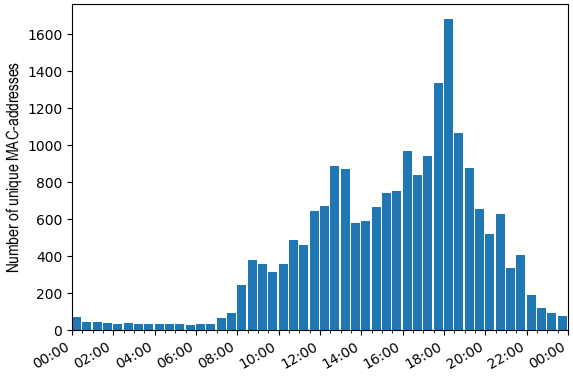
\includegraphics[width=0.38\textwidth]{img/daySum.png} 
    \caption{Unique Mac-addresses seen over time on an average weekday (bin size 30 minutes)}
    \label{fig:WeekdayHist}
\end{figure}

During the weekend it is expected that the shopping audiences will be more spread out over the day. This as less people have to work during the weekend and more people do leisure shopping. Because the sniffer is stationed at the entrance, also people passing by (but not entering) are detected.

looking at Figure \ref{fig:SaturdayHist} it can be seen that the customer activity observed around 8:30 is less than half compared to a weekday. However from 12:00 until 19:00 there are at least 1000 unique MAC addresses at any given time. Another interesting observation is that for both work and weekdays there is a small peak right before closing time of people who last minute need to buy something before closing time. 
\begin{figure}[h!]
    \centering
    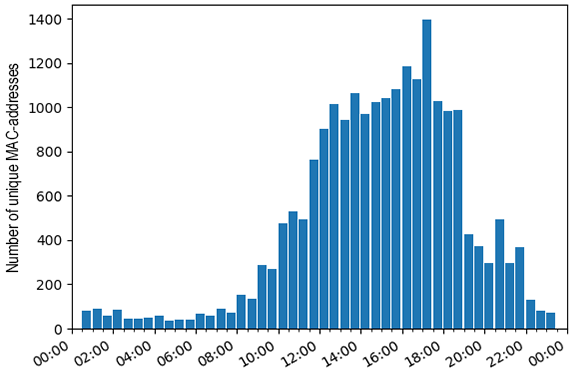
\includegraphics[width=0.4\textwidth]{img/daySat.png} 
    \caption{Unique Mac-addresses seen over time on an average weekend day (bin-size 30 min)}
    \label{fig:SaturdayHist}
\end{figure}

\subsubsection{Mac randomization as a privacy enhancing feature}
As a privacy-feature, smart phones running the latest versio of Android or Ios have the possibility to randomize their mac address when sending probe requests. However this option is not always turned on by default. By observing large amounts of probe requests over the span over several days reoccurring mac addresses can be identified and separated from MAC addresses that are only seen once. From the 91662 at least 5200 MAC addresses were seen with intervals of at least 24 hours in between sightings. This indicates that at least 5200 smart phones do not utilizes MAC spoofing when probing for APs. It is hard to do any estimates on the proportion of spoofing versus non-spoofing since it is very hard to tell how many of the 91622 MAC addresses belong to the same smart phone. Further because the data was only monitored for a week it is possible that from the 91662 addresses a subset does not utilize MAC spoofing but has not visited the store multiple times during that week. 
Attempts were made to inspect the probe request header to try and link multiple MAC addresses to a single origin. But since the header only contains meta data on supported rates and radio information this was very hard to do. Mainly because these values are the same per model of a phone, and are the same for devices using the same System-on-a-chip IC. Other common options for OS-fingerprinting rely on certain behavior embedded in for example TCP data, but since we are not associated with a Wi-Fi AP we were not able to extract this data from the packets.

The reoccurring MAC addresses can be correlated with costumer loyalty programs like the 'bonus-kaart'. This would give shops the possibility to track costumers based on mac address. With multiple access-points in the store, it would be possible to locate and find the interests of the costumer. Even with randomized mac addresses it would be possible to measure the average time people spend in front of certain shelf's. As this tracking technique is passive it is undetectable by the client. Only a limited amount of phones randomize there MAC address and people are unaware of the setting being enabled or not. The combination of these points makes it almost impossible to find out if one is being tracked or not. For now, turning Wi-Fi off is the only way to prevent this kind of tracking. 

\begin{figure}[h!]
    \centering
    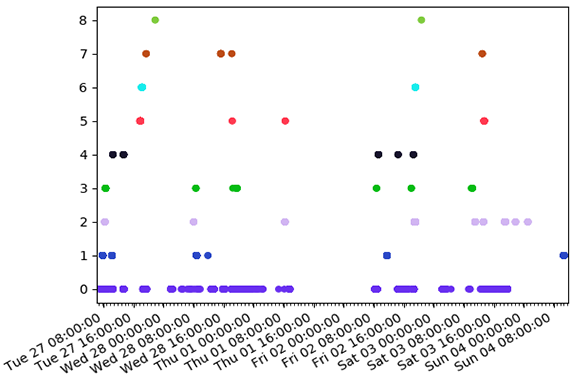
\includegraphics[width=0.4\textwidth]{img/selectedmac.png} 
    \caption{Selected Mac-addresses seen over 5 days (missing data from Thursday)}
    \label{fig:selected}
\end{figure}

To test the possibilities of MAC address tracking, the authors own mac-addresses and 6 other interesting mac addresses were filtered out (see figure \ref{fig:selected} above). The results correspond with a personal log-book tracking when one of the authors was near the sniffer. The purple color MAC address (at line 0 in the graph) corresponds with the MAC address of the phone of J. Brouwer, who lives within the range of the sniffer. Figure \ref{fig:selected} clearly shows when J. Brouwer was home or not. From the original data it was even possible to determine when he was sleeping, as his phone entered a sleeping mode resulting in less probes per minute when not being used over a long period of time.

The black colored mac address (line 4 in the graph) corresponds with the mac address of the phone of N. Hokke. These data-points show when N. Hokke went near the sniffer, either to shop or pick to up J. Brouwer to go study. Furthermore the person connected to MAC address 5 seems to visit the store every day except Friday, and either in the morning around 8:30 or in the evening around 18:00 on weekdays. On Saturday this person visited the store around 13:30. 

\subsection{Market share by Vendor}
Although not related to activity tracking, the authors thought it would be interesting to also plot the market share per vendor based on the recorded data, as this data is embedded in the MAC address anyway. The market share of the 6 most seen vendors are displayed in Figure \ref{fig:piechart}

\begin{figure}[h!]
    \centering
    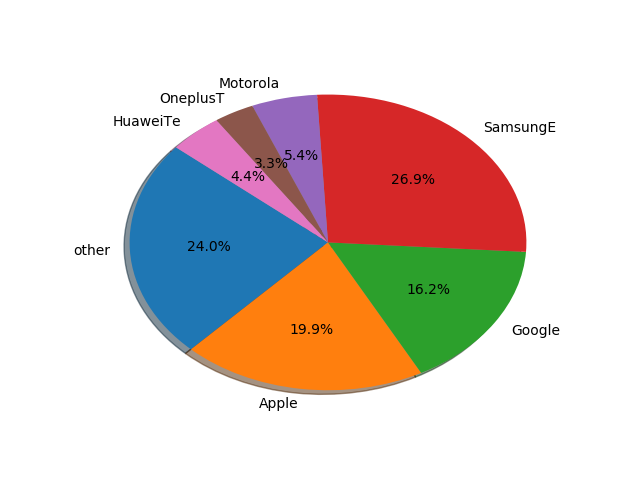
\includegraphics[width=0.4\textwidth]{img/piechard.png} 
    \caption{Pi chart of market share by vendor}
    \label{fig:piechart}
\end{figure}


\section{Conclusion and further work}
With the use of probe requests it was possible to create an activity graph of a grocery store that matches our expectations and can be used to distinguish working days from weekend days. Doing basic individual analysis it was possible to accurately determine when one of the authors was home, got picked up by the other author and even determine the author's sleeping pattern based on low activity of the phone. Also individual shopping behavior of random customers could be tracked.
Future research goals might include spoofing an access point known to a lot of people (e.g. university Wi-Fi or the free Wi-Fi supplied by public transport) to bypass MAC randomization. As a phone will use its real MAC address when trying to associate with known networks. It might also be worthwhile to not only scan for Wi-Fi traffic, but also scan and try to correlate it with Bluetooth traffic.


% conference papers do not normally have an appendix


% use section* for acknowledgment

% trigger a \newpage just before the given reference
% number - used to balance the columns on the last page
% adjust value as needed - may need to be readjusted if
% the document is modified later
%\IEEEtriggeratref{8}
% The "triggered" command can be changed if desired:
%\IEEEtriggercmd{\enlargethispage{-5in}}

% references section

% can use a bibliography generated by BibTeX as a .bbl file
% BibTeX documentation can be easily obtained at:
% http://mirror.ctan.org/biblio/bibtex/contrib/doc/
% The IEEEtran BibTeX style support page is at:
% http://www.michaelshell.org/tex/ieeetran/bibtex/
%\bibliographystyle{IEEEtran}
% argument is your BibTeX string definitions and bibliography database(s)
%\bibliography{IEEEabrv,../bib/paper}
%
% <OR> manually copy in the resultant .bbl file
% set second argument of \begin to the number of references
% (used to reserve space for the reference number labels box)
\begin{thebibliography}{1}

\bibitem{SmartPenetration}
NewsZoo, \emph{Global Mobile Market Report}, 2017

\bibitem{ProbeFrequency}
Julien Freudiger, \emph{How Talkative is your Mobile Device? An Experimental Study of Wi-Fi Probe Requests}, WiSec’15 June 22-26 2015, New York City, NY, USA

\bibitem{chanhop.sh}
codegist user: hnw \emph{http:\/\/codegists.com\/snippet\/shell\/chanhopsh\_hnw\_shell}

\end{thebibliography}

\onecolumn

{Appendix A}


\begin{figure}[h!]
    \centering
    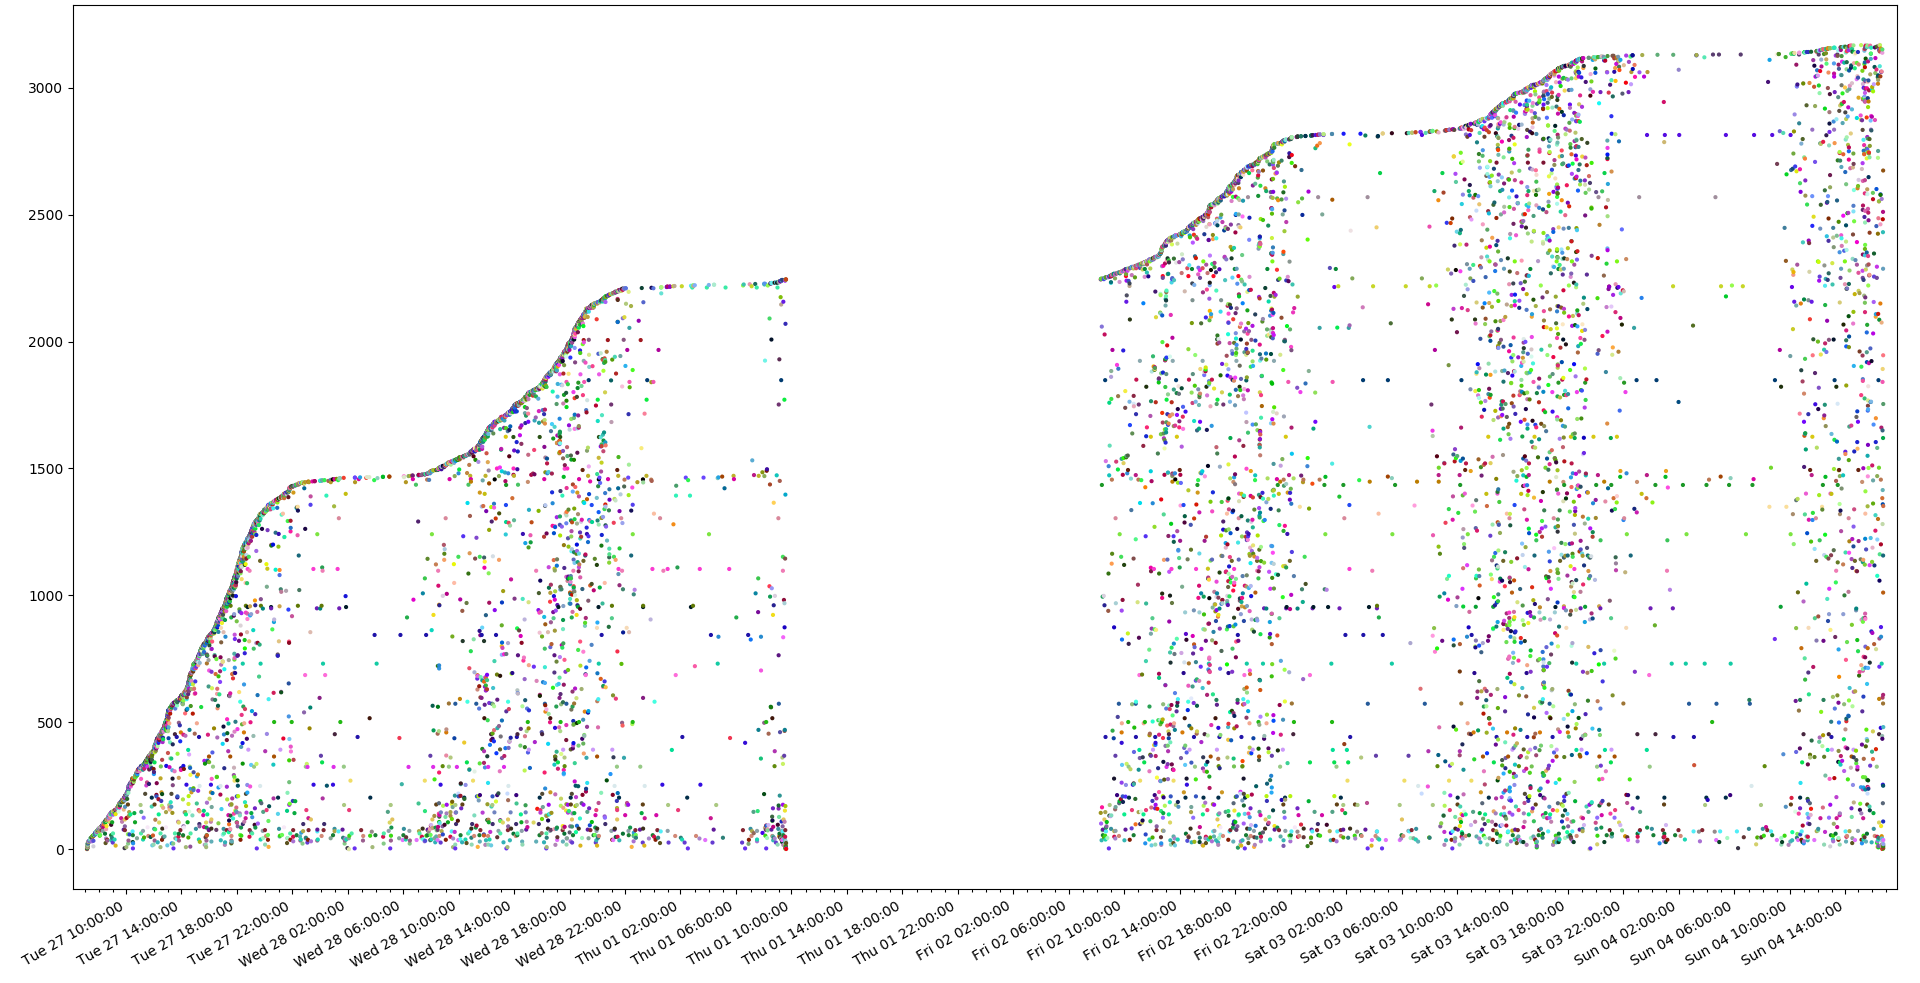
\includegraphics[width=1\textwidth]{img/Macovertime.png} 
    \caption{When plotting the last three bytes were used as RGB values for the dot to give the same MAC addresses the same color. the plot was made from left to right, meaning that if the a new mac appeared it would generate a new Y value, if it already existed it would be plotted on a lower. As a result every dot that is not the highest for that given time is a MAC that has been seen before }
    \label{fig:mactime}
\end{figure}





% that's all folks
\end{document}


